\documentclass[11pt, a4paper]{article}
\usepackage[slantfont, boldfont]{xeCJK}
\usepackage{ulem}
\usepackage{amsmath}
\usepackage{booktabs}
\usepackage{colortbl}
\usepackage[top = 1.0in, bottom = 1.0in, left = 1.0in, right = 1.0in]{geometry}
\usepackage{lipsum}
\usepackage{graphicx}
\usepackage{hyperref}
\usepackage{listings}
\usepackage{xcolor}
\usepackage{indentfirst}
\usepackage{mdwlist}
\usepackage{enumerate}


% \setCJKmainfont{SimSun}
% \setCJKmonofont{SimSun}
\setCJKmainfont{PingFang SC}
\setCJKmonofont{PingFang SC}

% \setmainfont[BoldFont={SimHei},ItalicFont={KaiTi}]{SimSun}
% \setsansfont[BoldFont=SimHei]{KaiTi}
% \setmonofont{Consolas}
\setmonofont{Menlo Regular}

\setlength{\parskip}{0.5\baselineskip}
\setlength{\parindent}{2em}

\newcolumntype{Y}{>{\columncolor{red}}p{12pt}}
\newcolumntype{N}{>{\columncolor{white}}p{12pt}}

\title{设计实现 Tomasulo 调度算法~实验报告}

\author{计55 王逸松 2015011369 \\ \\ 计54 陈宇 2015011343}
% \date{}
% \title{???}
% \author{???}


% \lstset{numbers=left,
% numberstyle=\tiny,
% keywordstyle=\color{blue!70}, commentstyle=\color{red!50!green!50!blue!50},
% frame=shadowbox,
% rulesepcolor=\color{red!20!green!20!blue!20}
% }

\lstset{
  % language=[ANSI]c,
  basicstyle=\footnotesize\ttfamily,
  numbers=left,
  keywordstyle=\color{blue},
  numberstyle={\tiny\color{lightgray}},
  stepnumber=1, %行号会逐行往上递增
  numbersep=5pt,
  commentstyle=\small\color{red},
  backgroundcolor=\color[rgb]{0.95,1.0,1.0},
  showspaces=false,
  showtabs=false,
  frame=shadowbox, framexleftmargin=5mm, rulesepcolor=\color{red!20!green!20!blue!20!},
% frame=single,
%  TABframe=single,
  tabsize=4,
  breaklines=tr,
  extendedchars=false %这一条命令可以解决代码跨页时,章节标题,页眉等汉字不显示的问题
}


\begin{document}
\maketitle

\section{实验原理}

\subsection{Tomasulo 算法}

Tomasulo 算法是由 Robert Tomasulo 发明的。首先采用该方法的是 IBM360/91 机器中的浮点部件。

该算法以硬件方式实现了寄存器重命名,允许指令乱序执行。其结构如下图:

\begin{center}
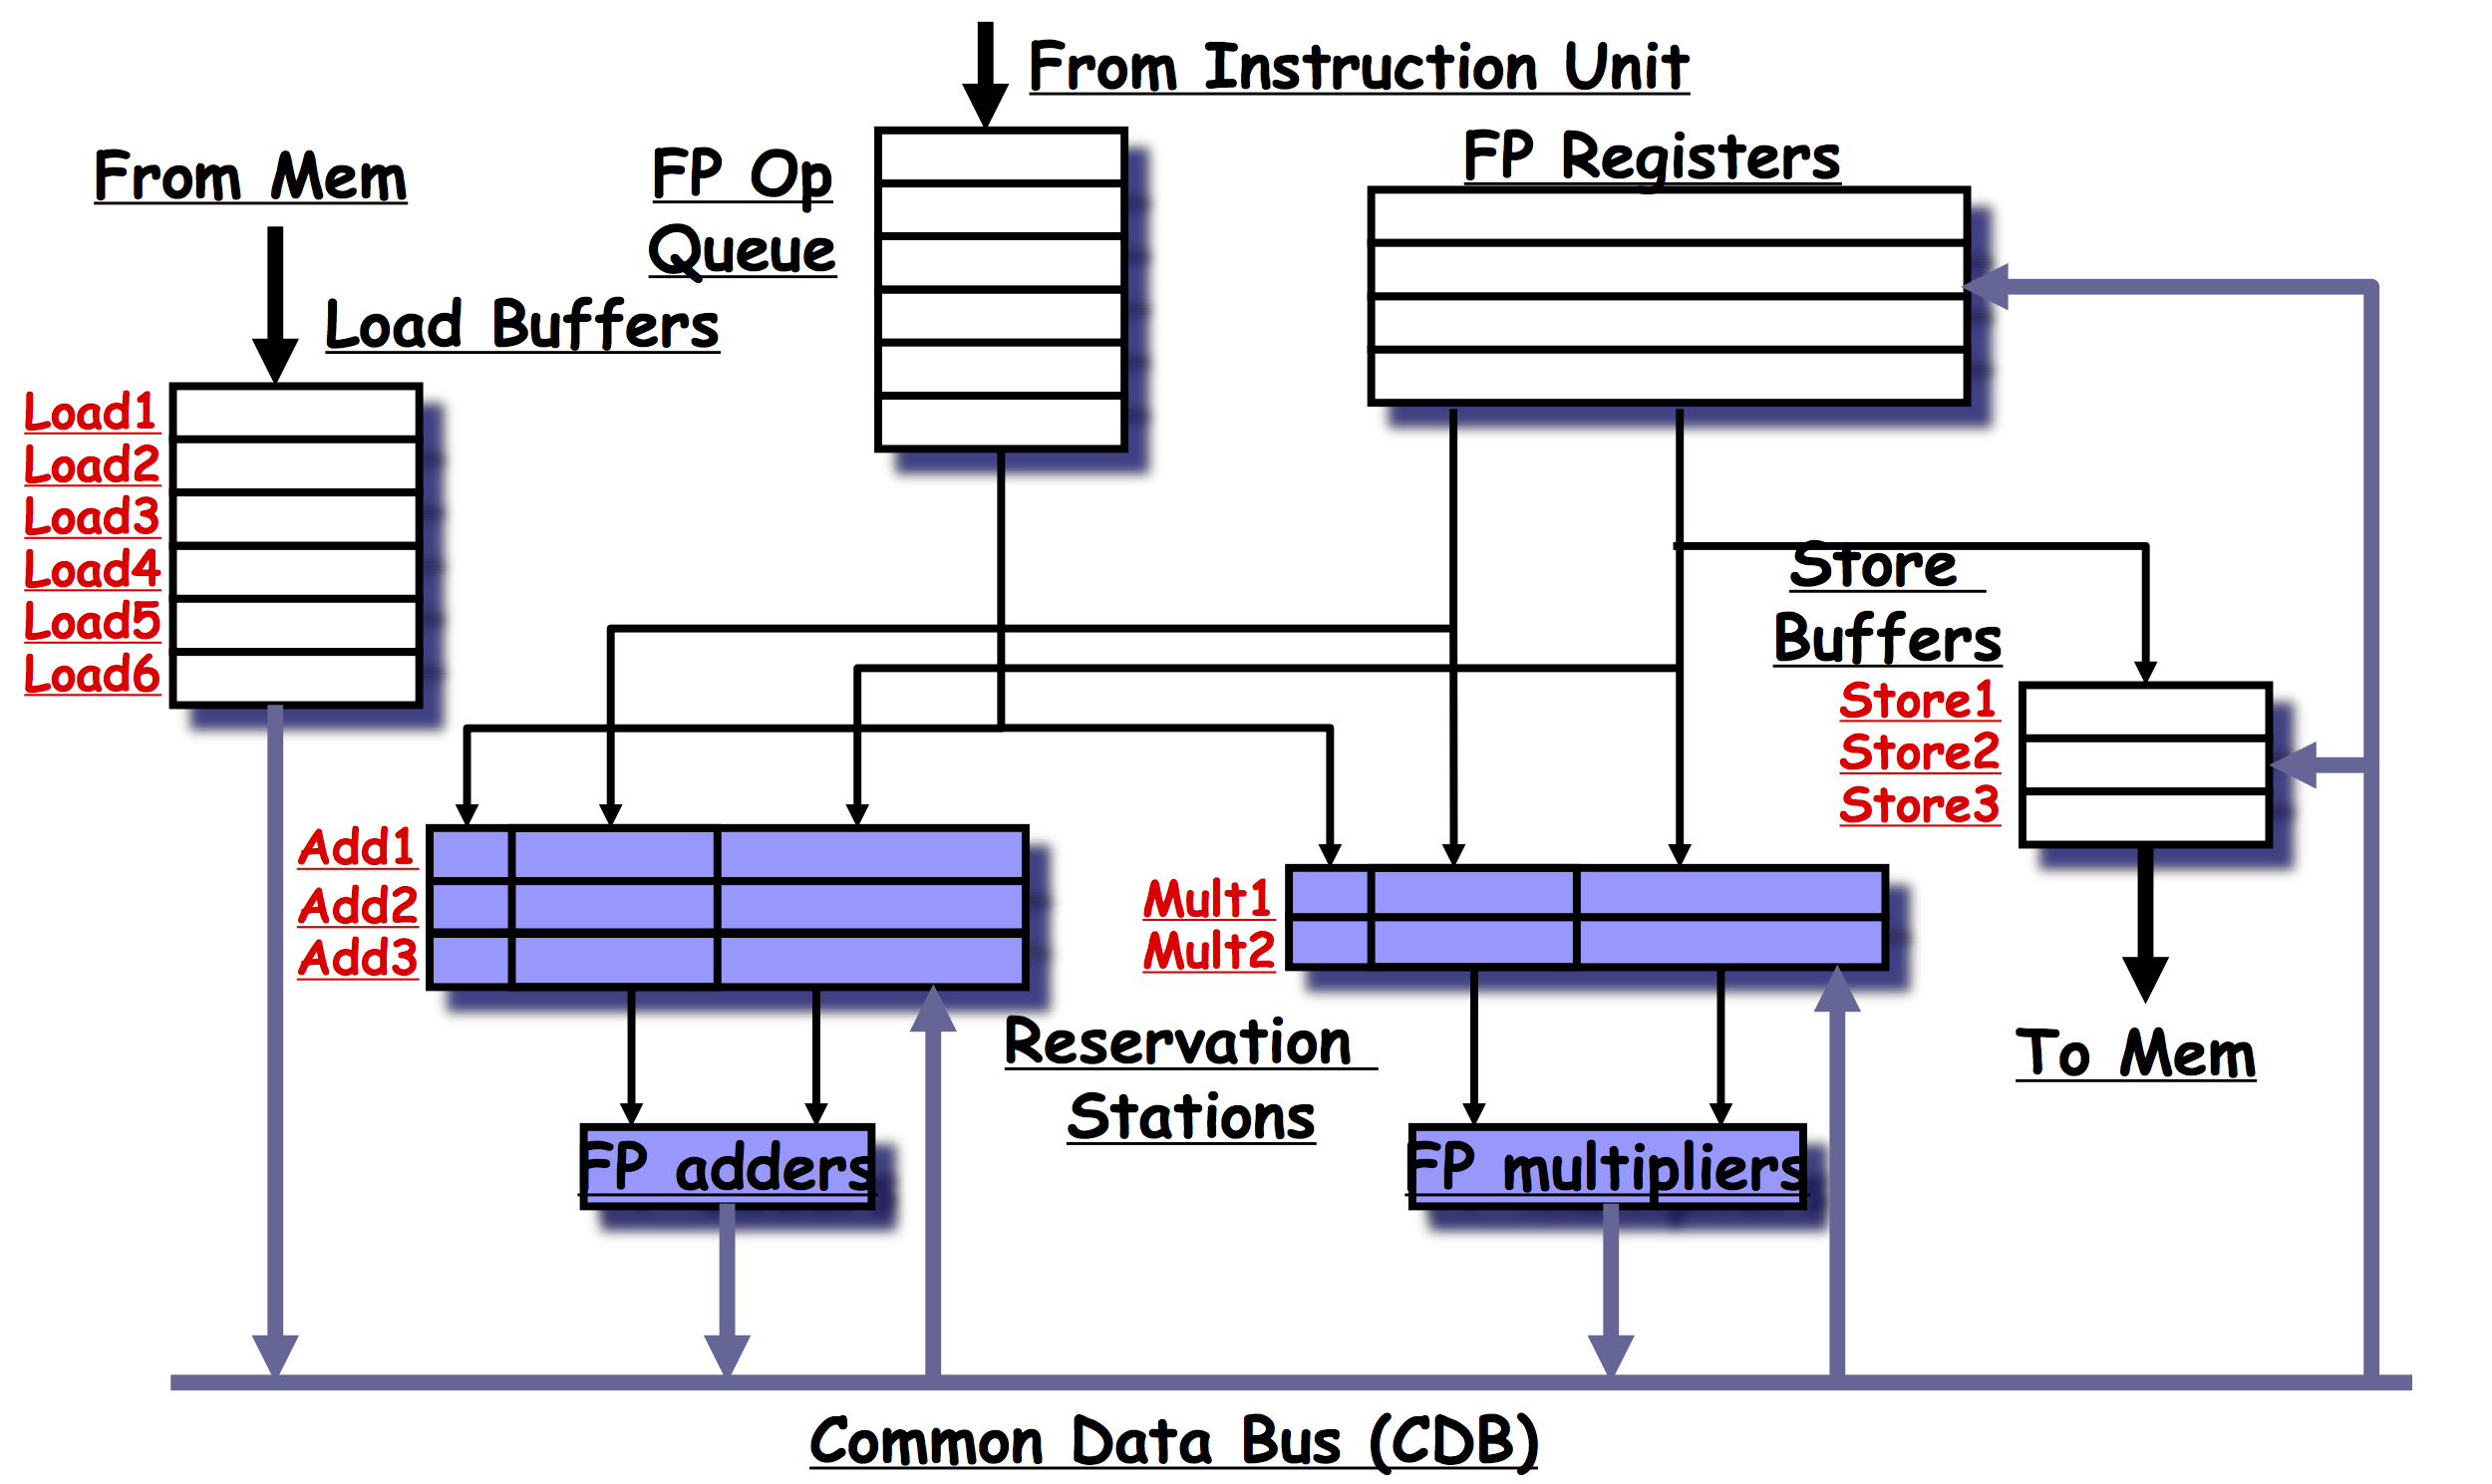
\includegraphics[width=350pt]{images/tomasulo-arch.png}
\end{center}

在每一个时钟周期,取指单元从内存中获取最多一条指令,并将其发射到相应的保留站。
对于访存指令,会被暂存到 Load/Store Buffer ;而对于浮点操作指令,会被暂存到浮点加法器或乘法器的保留站中。
当保留站的某条指令的源操作数都到齐,且对应的功能部件空闲时,这条指令便可以开始执行;而在访存队列中,为保证访存的正确性,必须以某种顺序来执行这些访存指令。
每条指令执行完成后,会尝试获得公共数据总线 (Common Data Bus) 的使用权,并广播其要写回的数据,以提供给其他指令使用。



\section{实验要求}

\begin{itemize}
  \item 设计实现 Tomasulo 算法模拟器,不限语言。
  \item {
    能够执行浮点加、减、乘、除运算以及 load 和 store 操作,具体如下:
    
    \begin{tabular}{|c|c|c|c|}
      \hline
      指令格式 & 指令说明 & 指令周期 & 保留站/缓冲队列项数 \\ \hline
      \texttt{ADDD F1, F2, F3} & \texttt{F1, F2, F3} 为浮点寄存器 & 2 个周期 & 3 \\ \hline
      \texttt{SUBD F1, F2, F3} & 同上 & 2 个周期 & 3 \\ \hline
      \texttt{MULD F1, F2, F3} & 同上 & 10 个周期 & 2 \\ \hline
      \texttt{DIVD F1, F2, F3} & 同上 & 40 个周期 & 2 \\ \hline
      \texttt{LD F1, ADDR} & $0 \le \texttt{ADDR} < 4096$ & 2 个周期 & 3 \\ \hline
      \texttt{ST F1, ADDR} & 同上 & 2 个周期 & 3 \\ \hline
    \end{tabular}
    
    其中浮点加法器为两段流水线,浮点乘除法器的流水线可以自行设计。
  }
  \item {
    支持单步执行和连续执行,实时显示算法的运行状态,
    包括各条指令的运行状态、各寄存器以及内存的值,保留站和 Load/Store Buffer 的状态等。
  }
  \item {
    提供数据输入和指令输入的功能。
  }
\end{itemize}


\section{设计实现}

为了方便跨平台运行和降低开发难度,我们采用了 HTML 和 JavaScript 等语言来实现。

\subsection{显示界面}

我们用 HTML 和 JavaScript 来实现显示界面,使用了 Bootstrap 和 jQuery 等框架和库。
运行时截图如下:

\begin{center}
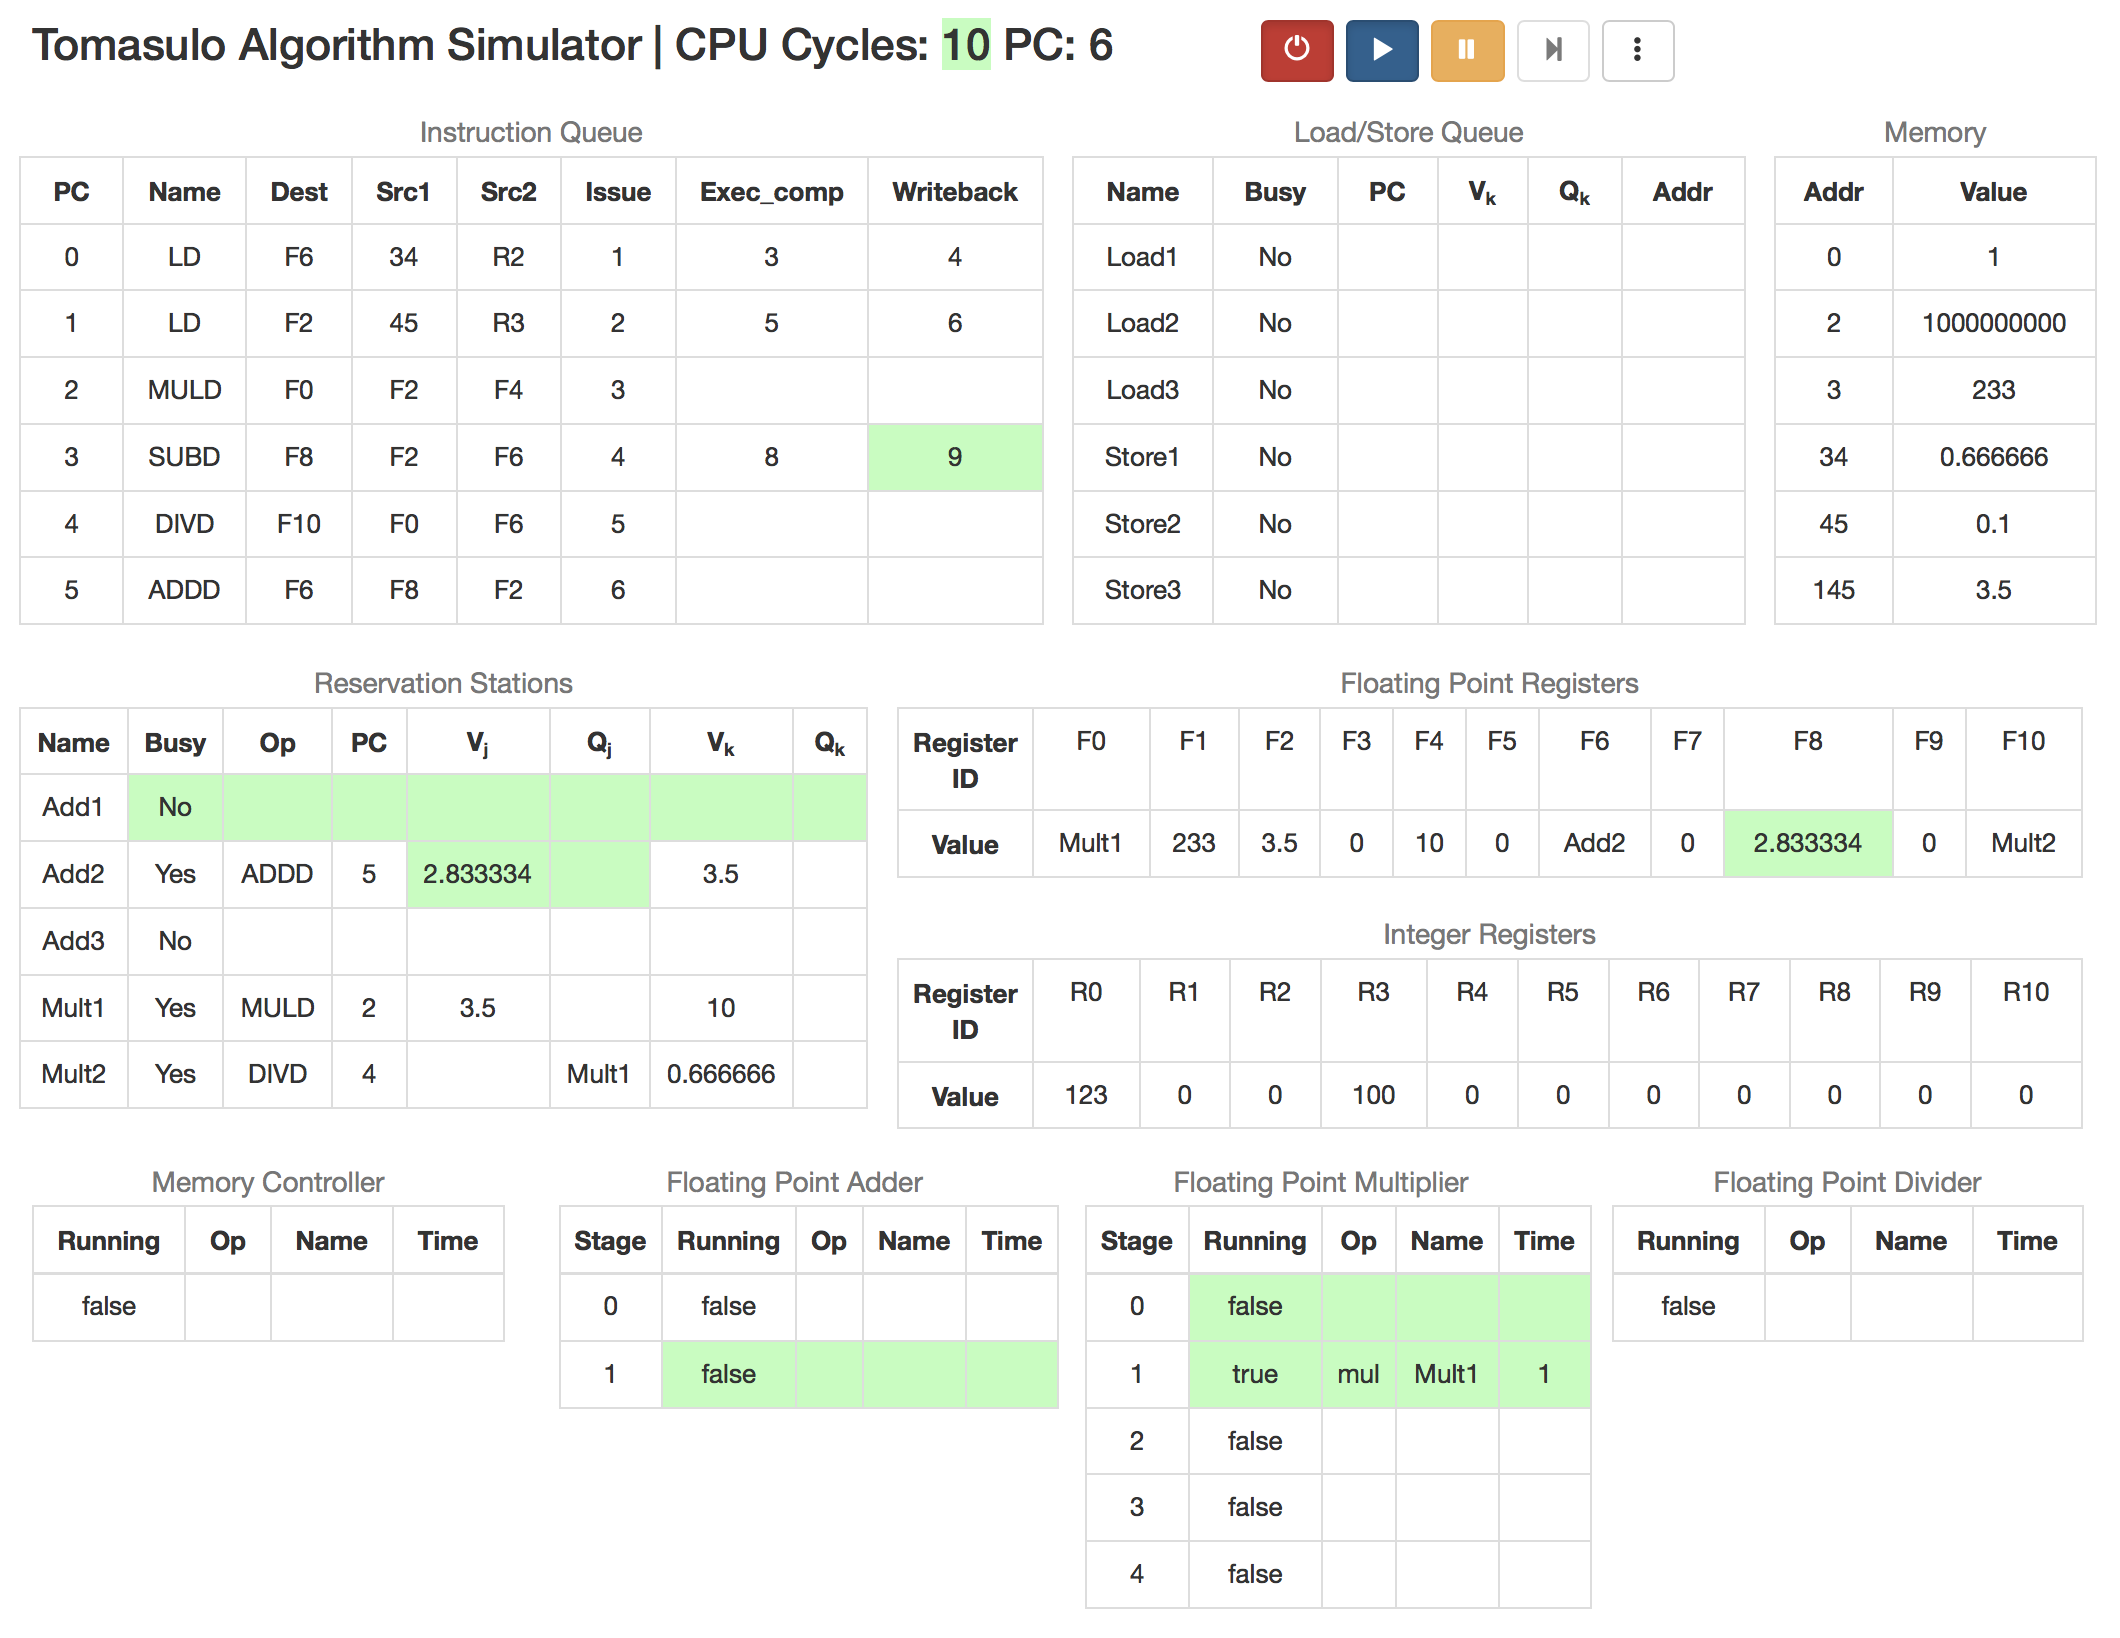
\includegraphics[width=400pt]{images/screenshot-1.png}
\end{center}

其中各表格表示了 CPU 的各部件的运行状态,各按钮实现了对 CPU 的控制功能,具体使用方法见用户使用手册。

\subsection{CPU 的设计和实现}

CPU 的主体部分是在 \texttt{js/CPU.js} 文件中实现的。
在我们的实现中,CPU 的各项性能均与实验要求相一致,其中浮点乘法器为 5 段流水,每段 2 个时钟周期,浮点除法器不使用流水,需要 40 个时钟周期。

在实现过程中使用了不少编程技巧,其中最重要的一个为\textbf{硬件级模拟}:

为了在实现的过程中贴合硬件的思维方式,我们创建了一个 \texttt{HDL} 类,
其中的 \texttt{signal} 函数会返回一个对象,
该对象内部有一个变量,可以将其设置为一个新的值,但是要在时钟上升沿到来时才生效。
这个对象的行为与 \texttt{VHDL} 等硬件描述语言中的 \texttt{signal} ,或数字逻辑电路中的 D 触发器的行为类似。

得益于上述技巧,我们在 CPU 中实现了一些硬件中较为容易实现的特性:

\textbf{流水线旁路}

在硬件流水线中,旁路 (forwarding) 被经常使用,来解决各种冲突,或减少各种延迟。
由于我们的 CPU 的各数据都存在各 \texttt{signal} 中,实现旁路就像在硬件中实现一样简单。
事实上,CPU 时钟周期内的代码可以很方便的翻译成各硬件描述语言。

\textbf{内存控制器}

对于 load 和 store 指令,为了保证其访存行为正确,
我们采用的是最保守的方法,即严格按照指令顺序执行它们。
为此,我们实现了一个硬件的“内存控制器” (memory controller) ,
每个时钟周期会找到所有待执行的 load 和 store 指令中,
PC 最小的一条,并尝试执行它。

由于内存控制器的存在,所有访存指令必须按序执行,且一条执行完了才能执行下一条,
这使得在一些测试数据中,与教材和课件上的结果不一致,但是 load 指令的确是“2 个周期”的。


\section{实验心得}

这是我们本学期做过的最后一个作业,也是代码量最大的一个作业(2000+ 行)……


\includegraphics{images/facepalm-1.png}

总体来说感觉不错,并且收获很大。比如说从零开始掌握了 Tomasulo 算法,比如说为了写 UI 从零开始学会了 Bootstrap 等框架。

在细节上,我认为比较好的是,通过对该算法的完整实现和艰难的调试,以及编写详细的用户使用手册,我们对 Tomasulo 算法有了更深入的理解。

我认为不足的,一方面是说,教材和课件给的\textbf{解释不够清晰},\textbf{例子比较少},一些细节只能由我们自己推敲,最终没能完全跟课件上的样例达成一致,
以及助教在 deadline 之前三天突然修改了对“流水线”的解释,使我们受到不小的压力。

另一方面,在对比国外大学的课件之后,我认为本课程对该算法的一些细节问题,并\textbf{没有做充分的讨论},
比如说 CMU 的计算机系统结构课程中,讲完 Tomasulo 算法之后,对很多问题进行了深入的讨论,比如访存顺序问题如何解决,提出了三种方案让我们思考等等,
而在本课程中尚未提及。当然,我个人的观点是,\textbf{国内课业压力比较大},学生们也很难拿出时间进行这样的研究学习。



\section*{参考资料}

\begin{enumerate}[{[}1{]}]
  \item 张晨曦,王志英,计算机系统结构教程(第2版),北京:清华大学出版社,2014
  \item ``Bootstrap · The world's most popular mobile-first and responsive front-end framework.", http://getbootstrap.com
  \item ``jQuery'', https://jquery.com
  \item Prof. Onur Mutlu, ``Lecture 13: Out-of-Order Execution and Data Flow'', Carnegie Mellon University
\end{enumerate}


\end{document}
